%\def\xxactivite{Tris}
%
%\def\xxauteur{Emilien Durif -- Xavier Pessoles}
%\fichefalse \proftrue \tdfalse \courstrue
%
%\def\xxnumchapitre{Chapitre 8 \vspace{.2cm}}

\section{Tris}
\subsection{Introduction et objectifs}

\marginnote{
\begin{itemize}
\item algorithmique quadratique : tri par insertion, par sélection;
\item tri par partition-fusion;
\item tri par comptage.
\end{itemize}}


\begin{obj}
%On suppose dans toute la suite que l'on trie des tableaux dans l'ordre croissant. Les algorithmes présentés permettent de trier n'importe quel type d'éléments à partir du moment où ces éléments sont munis d'un ordre total. Cependant nous allons nous focaliser ici sur le tri d'entiers.

Un algorithme de tri est un algorithme permettant d'organiser une liste d'éléments selon un ordre fixé.  On peut dire que les éléments à trier feront partie d'un ensemble $E$ muni d'une relation d'ordre total noté $\leq$.

Les ensembles $\mathbb{N}$, $\mathbb{R}$... sont munis de l'ordre $\leq$. 

L'ensemble des chaînes de caractères peut être muni de l'ordre lexicographique (ordre du dictionnaire). Ainsi en Python, \texttt{'a'<'b'}, \texttt{'aa'<'b'}, \texttt{'A'<'a'} (les lettres majuscules sont avant les lettres minuscules).

Les principales capacités développées ici sont :
\begin{itemize}
\item comprendre un algorithme de tri et expliquer ce qu'il fait;
\item s'interroger sur l'efficacité algorithmique temporelle d'un algorithme;
%\item Distinguer par leurs complexités deux algorithmes résolvant un même problème.
\item programmer un algorithme dans un langage de programmation moderne et général.
\end{itemize}

\end{obj}




\begin{defi}[Effet de bord] On dit qu'une fonction est à effet de bord lorsqu'elle modifie une variable  en dehors de son environnement local. C'est par exemple le cas lorsqu'on donne une liste (objet mutable, passé par référénce) comme argument d'une fonction.

Conséquence sur les algorithmes de tri : une fonction de tri ne renvoie rien la plupart du temps (on peut donc l'appeler une procédure). La liste passée en argument en entrée sera triée et cela, même en dehors du scope de la fonction. 
\end{defi}


\begin{defi}[Tri en place]
Un tri est effectué en place lorsque la liste à trier est modifiée jusqu'à devenir triée. Dans le cas contraire, la fonction de tri pourra renvoyer une novelle liste contenent les mêmes éléments, mais triés. 
\end{defi}


\begin{defi}[Tri stable]
Un algorithme est dit stable si les positions relatives de deux éléments égaux ne sont pas
modifiées par l'algorithme : c'est-à-dire que si deux éléments $x$ et $y$ égaux se trouvent aux positions $i_x$ et $i_y$ de
la liste avant l'algorithme, avec $i_x < i_y$, alors c'est également le cas de leurs positions après l'algorithme.
% Le caractère stable peut-être utile lorsqu’on utilise des pré-ordres.
\end{defi}

\begin{defi}[Tri comparatif]
Un tri est dit comparatif lorsqu'il s'appuie uniquement sur la comparaison deux à deux des éléments de la liste et pas sur la valeur ce ces éléments.
\end{defi}





\begin{marginfigure}
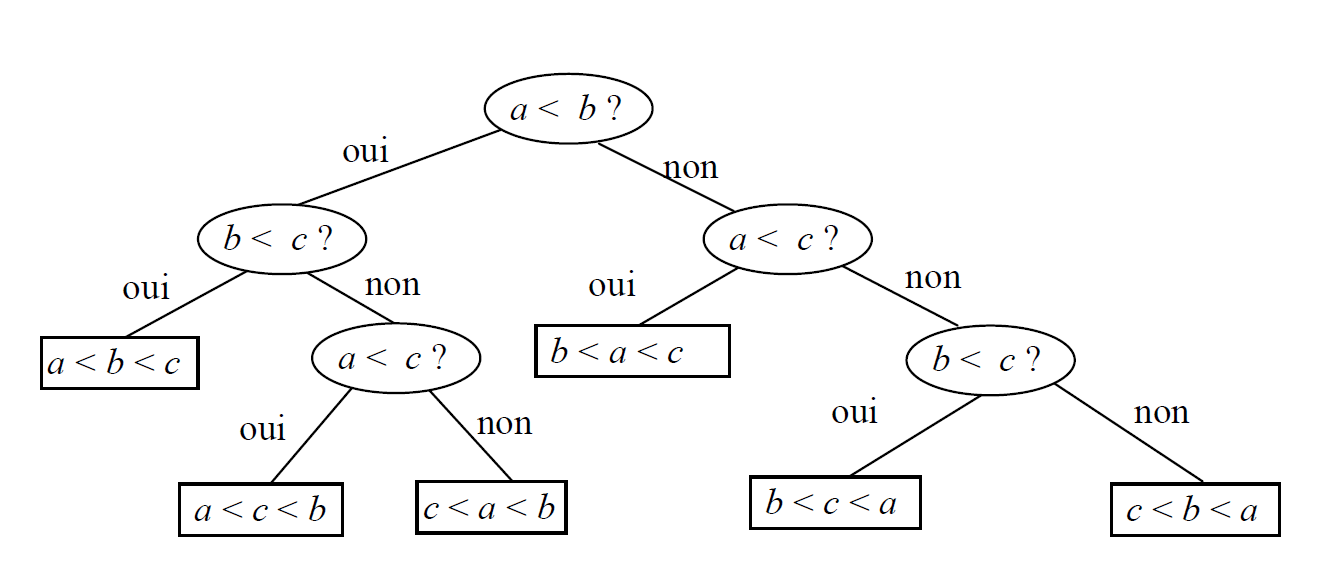
\includegraphics[width=\textwidth]{C2.png}
\end{marginfigure}
\begin{exemple}%{Tri comparatif}

Un \textbf{algorithme comparatif} (à opposer au non-comparatif comme le tri baquet ou par paquet) est basé sur des comparaisons successives entre les données pour déterminer la permutation correspondant à l'ordre croissant des données.
On va chercher ici à évaluer la complexité théorique des tris comparatifs en se basant sur le nombre de comparaisons.

Cet algorithme correspond au fonctionnement du tri insertion que nous verrons plus loin.

%\textbf{Résultat :}\textit{ Tout algorithme comparatif fait dans le pire des cas au moins de l'ordre de
%\textbf{$n \log_2(n)$ comparaisons} soit une complexité de \textbf{$O(N\cdot \log(N))$}}.
\end{exemple}

\subsection{Tri par insertion}
\subsubsection{Principe}

\begin{defi}[Principe du tri par insertion]
Le \textbf{tri par insertion} est le tri que l'on effectue naturellement, par exemple pour trier un jeu de cartes. On trie les premières puis à chaque nouvelle carte on l'ajoute à l'ensemble déjà trié à la bonne place. 

Ce tri s'effectue en place, c'est-à-dire qu'il ne demande pas d'autre tableau que celui que l'on trie. 

Son coût en mémoire est donc constant si on ne compte pas la place occupée par les données.
\end{defi}



\subsubsection{Implémentation}


\begin{itemize}
\item On stocke les données dans un tableau $L$ entre les indices $0$ et $n-1$.
\item On utilise deux variables notées $i$,$j$ et une variable \texttt{clef} (la clef) du même type que les données de la liste.
\item On réalise une première boucle qui va permettre de parcourir tous les éléments $L[i]$ du tableau à trier.
Chacun de ces éléments sera alors successivement la clef.
\item La deuxième boucle (\texttt{while}) va nous permettre pour chaque valeur de la clef de tester successivement les valeurs déjà triées jusqu'à trouver une valeur inférieure. On aura ainsi déterminé la place de la clef.
\item A chaque fois qu'une valeur est plus grande que la clef on la décale vers la droite pour laisser la place d'écrire la clef.
Dès que l'on arrive sur une valeur inférieure on a trouvé la bonne place pour écrire la clef.
\end{itemize}


\begin{lstlisting}
def tri_insertion(L:[int]) -> [int]:
    """
    Tri par insertion d'une liste d'entiers L.
    """
    n = len(L)
    for i in range(1,n):
        # Invariant : en entrée de boucle L[0:i-1] est triée.
        j = i
        v = T[i]
        while j>0 and v<L[j-1] :
            L[j] = L[j-1]
            j = j-1
        L[j] = v
        # Invariant : en fin de boucle L[0:i] est triée.
	
    return L # Le tri est en place, on n'est pas obligé de renvoyer L. 
\end{lstlisting}    


\subsubsection{Terminaison}

Pour la boucle \texttt{while}, la quantité \texttt{j} est un variant de boucle. En effet :
\begin{itemize}
\item avant d'entrer dans la boucle, \texttt{j} est une quantité entière strictement positive;
\item \texttt{j} est décrémenté de 1 à chaque itération, donc \texttt{j} décroit strictement à chaque itération. 
\item \texttt{j} est donc un variant de boucle.
\end{itemize}


La boucle \texttt{for} termine au bout de \texttt{n-1} itérations. L'algorithme de tri par insertion termine donc.

\subsubsection{Correction}
Montrons que la propriété \texttt{L[0:i] est triée} est un invariant de boucle.

\textbf{Initialisation} 
En entrant dans la boucle : \texttt{i=1}; donc \texttt{L[0:1]} ne contient qu'un élément. \texttt{L[0:1]} est triée.

\textbf{Hypothèse} : considérons qu'au début de l'itération \texttt{i}, \texttt{L[1:i-1]} est triée. 

Montrons qu'à la fin de l'itération \texttt{i}, \texttt{L[1:i]} est triée. 
\begin{itemize}
\item \texttt{v = L[i]} est la valeur à insérer dans \texttt{L[0:i-1]}.
\item \textbf{ou bien} \texttt{v>=L[i-1]}, on n'entre pas dans la boucle \texttt{while} et \texttt{L[i]=v}; donc \texttt{L[0:i]} est triée. 
\item \textbf{ou bien} \texttt{v<L[i-1]} et on entre dans la boucle \texttt{while}.\texttt{j} décrémente alors et tous les éléments sont << décalés vers la droite >>  jusqu'à ce que \texttt{v>=L[j-1]}. On insère alors \texttt{v} en \texttt{L[j]}.
\end{itemize}

À la fin du \texttt{n-1} tour de boucle, \texttt{L[0:n]} est donc triée. 


\subsubsection{Complexité}

\begin{prop}[Complexité]
%\begin{itemize}
%\item La fonction $tri\_insertion$ effectue le même nombre de comparaisons et d'affectations. Lorsque la boucle while insère l'élément $T[i]$ à la position $i-k$, elle effectue $k+1$ comparaisons. 
%
%
%\item \textbf{Dans le meilleur des cas} le tableau est déjà trié. 
%La valeur clef est donc forcément plus grande que toutes les précédentes. Dès la première comparaison on s'arrête: 
%$k$ vaut $0$.
%Soit une comparaison par boucle while réalisée, il y a donc $n-1$ comparaisons à effectuer au total. La complexité est donc de classe linéaire : $C(n)=O(n)$.
%
%\item \textbf{Dans le pire des cas}, le tableau est trié à l'envers. La valeur clef est donc forcément plus petite que toutes les précédentes.
%Il faut donc comparer et décaler toutes les valeurs précédentes jusqu'à mettre la valeur clé en première position:  $k$ vaut $i$, avec $i$ qui varie de $1$ à
%$n-1$.
%\item On en déduit donc un nombre total de $\frac{n\times(n-1)}{2}$ comparaisons (somme d'une suite arithmétique).
%\end{itemize}


\textbf{La complexité est dans le pire des cas quadratique : $C(n)=\mathcal{O}(n^2)$.}

\textbf{La complexité est dans le meilleur des cas linéaire : $C(n)=\mathcal{O}(n)$.}
 

L'efficacité du tri par insertion est excellente lorsque le tableau est déjà trié ou « presque trié » $(C(n)=\mathcal{O}(n))$. 

Il surpasse alors toutes les autres méthodes de tri qui sont au mieux en $\mathcal{O}(n \times \ln(n))$.
\end{prop}


Au vu de notre algorithme, le pire des cas que l'on peut rencontrer est celui où la liste \texttt{L} est triée dans l'ordre décroissant. En effet, dans ce cas, à l'itération \texttt{i}, la boucle while devra être réalisée \texttt{i} fois. 

Comptons le nombre de comparaisons \texttt{j>0} réalisées par l'algorithme pour une liste de \texttt{n} éléments :
\begin{itemize}
\item à l'itération 1 : il y a 2 comparaisons; 
\item à l'itération 2 : il y a 3 comparaisons; 
\item ...
\item à l'itération \texttt{n-1} : il y a \texttt{n} comparaisons.
\end{itemize}

Au final le nombre de comparaisons est égal à $C(n) = 2+3+...+n = \sum \limits_{i=1}^n \left(i\right)  -1 = \dfrac{1}{2}n\left(n+1\right) -1 = \mathcal{O}(n^2)$.







%
%
%%\subsection{Complexité}
%%
%%\begin{prop}{Complexité}
%%\begin{itemize}
%%\item La fonction $tri\_insertion$ effectue le même nombre de comparaisons et d'affectations. Lorsque la boucle while insère l'élément $T[i]$ à la position $i-k$, elle effectue $k+1$ comparaisons. 
%%
%%
%%\item \textbf{Dans le meilleur des cas} le tableau est déjà trié. 
%%La valeur clef est donc forcément plus grande que toutes les précédentes. Dès la première comparaison on s'arrête: 
%%$k$ vaut $0$.
%%Soit une comparaison par boucle while réalisée, il y a donc $n-1$ comparaisons à effectuer au total. La complexité est donc de classe linéaire : $C(n)=O(n)$.
%%
%%\item \textbf{Dans le pire des cas}, le tableau est trié à l'envers. La valeur clef est donc forcément plus petite que toutes les précédentes.
%%Il faut donc comparer et décaler toutes les valeurs précédentes jusqu'à mettre la valeur clé en première position:  $k$ vaut $i$, avec $i$ qui varie de $1$ à
%%$n-1$.
%%\item On en déduit donc un nombre total de $\frac{n\times(n-1)}{2}$ comparaisons (somme d'une suite arithmétique).
%%\end{itemize}
%%\textbf{La complexité est donc de classe quadratique : $C(n)=O(n^2)$.}
%%
%%
%%\begin{center}
%%\begin{tabular}{|c|c|c|}
%%\hline 
%%\rule[-1ex]{0pt}{2.5ex}  & meilleur cas &  pire cas \\ 
%%\hline 
%%\rule[-1ex]{0pt}{2.5ex} comparaisons & $N$ & $N^2/2$ \\ 
%%\hline 
%%\rule[-1ex]{0pt}{2.5ex} affectations & $N$ & $N^2/2$ \\ 
%%\hline 
%%\end{tabular} 
%%\end{center}
%%
%%
%%
%%L'efficacité du tri par insertion est excellente lorsque le tableau est déjà trié ou « presque trié » $(C(n)=O(n))$. Il surpasse alors toutes les autres méthodes de tri qui sont au mieux en $O(n \times ln(n))$.
%%\end{prop}
%
\subsection{Tri rapide (ou << quicksort >>)}

\subsubsection{Principe}

\begin{defi}[Tri rapide]
\textbf{L'algorithme de tri rapide} fait partie de la catégorie des algorithmes « diviser pour régner ».

À chaque appel de la fonction tri on choisit une valeur \textbf{<< pivot >>}, par exemple le premier élément. On effectue une partition des élément à trier. Un premier groupe est constitué de valeurs inférieures au pivot  et un deuxième avec les valeurs supérieures.
Le pivot est alors placé définitivement dans le tableau.

On traite alors chacun des groupes de façon indépendante. On peut les traiter avec le même algorithme.
\end{defi}

%
%
%
%
%
%\begin{exemple2}[Illustration du tri rapide]
%
%
%On représente en :
%\begin{itemize}
%\item bleu, le pivot;
%\item vert, les valeurs triées;
%\item rouge, les valeurs de gauche d'une segmentation;
%\item jaune, les valeurs de droite d'une segmentation. 
%\end{itemize}
%
%
%
%\noindent\begin{tabular}{|p{10.cm}|c|ccccc|}
%\hline
%\hline \rowcolor{white}
%Tableau $T$ initial: 5 est le pivot & \cellcolor{bleuc}5 & 14 & 11 & 8 & 17 & 7 \\ 
%\hline 
%\hline \rowcolor{white}
%On partitionne pour trouver une partie droite (en jaune) et une partie gauche (en rouge). Sauf qu'ici il n'y aura pas de partie gauche car 5 est la plus petite valeur. 5 est donc à sa place définitive. & \cellcolor{bleuc}5 &\cellcolor{jaune} 14 & \cellcolor{jaune}11 & \cellcolor{jaune}8 & \cellcolor{jaune}17 & \cellcolor{jaune}7 \\ 
%\hline 
%\hline \rowcolor{white}
% & \cellcolor{vertc}5 & & & & & \\ \cline{2-3} \rowcolor{white}
% \multirow{-2}{10.cm}{On traite de façon indépendante les partie gauche et droite. Ici pas de partie gauche. On cherche alors les nouveaux pivots (ici 14). }
%&&\cellcolor{bleuc} 14 & \cellcolor{jaune}11 & \cellcolor{jaune}8 & \cellcolor{jaune}17 & \cellcolor{jaune}7 \\
%\hline 
%\hline \rowcolor{white}
% & \cellcolor{vertc}5  & &  & &&   \\ \cline{2-3} \rowcolor{white}
% \multirow{-2}{10.cm}{On segmente alors les parties droite et gauche autour du pivot 14 dont on a ainsi déterminé la position définitive. }
%&& \cellcolor{rougec}11 & \cellcolor{rougec}8 & \cellcolor{rougec}7&\cellcolor{vertc} 14& \cellcolor{jaune}17  \\
%\hline 
%\hline \rowcolor{white}
% & \cellcolor{vertc}5  & &  & &\cellcolor{vertc} 14&   \\
% \cline{2-3} \rowcolor{white}
%  &   & \cellcolor{bleuc}11&\cellcolor{jaune}8 & \cellcolor{jaune}7&&   \\ \cline{2-3} \rowcolor{white}
% \multirow{-3}{10.cm}{On traite de façon indépendante les partie gauche et droite. On recherche pour chacune le pivot (ici 11 et 17). }
%&&  &  & && \cellcolor{bleuc}17  \\
%\hline\hline
%\rowcolor{white}
% & \cellcolor{vertc}5  & &  & &\cellcolor{vertc} 14&  \cellcolor{vertc}17 \\
% \cline{2-3} \rowcolor{white} 
% &   & \cellcolor{rougec}8&\cellcolor{rougec}7 & \cellcolor{bleuc}11&&   \\  
%  \\
% \cline{2-3} \rowcolor{white}
%\multirow{-3}{10.cm}{Pour la chaine de pivot 11 on segmente mais il n'y a pas de partie droite. Le pivot 17 est seul dans sa chaine il est donc directement à la bonne position. } &&&&&&\\
%\hline\hline
%\rowcolor{white}
% & \cellcolor{vertc}5  & &  &\cellcolor{vertc}  11&\cellcolor{vertc} 14&  \cellcolor{vertc} 17 \\
% \cline{2-3} \rowcolor{white}
% \multirow{-2}{10.cm}{8 est pivot de la partie gauche. Ici pas de partie droite donc 11 est placé.. }  &  & \cellcolor{bleuc}8 &  \cellcolor{jaune}7&&  & \\ \cline{2-3} 
%\hline\hline
%\rowcolor{white}
% & \cellcolor{vertc}5  & &  &\cellcolor{vertc} 11&\cellcolor{vertc} 14&  \cellcolor{vertc} 17 \\
% \cline{2-3} \rowcolor{white}
% \multirow{-2}{10.cm}{On segmente la chaine de pivot 8 Seul 7 est dans la partie gauche}  &   &\cellcolor{rougec}7 &\cellcolor{bleuc} 8 &&&   \\ \cline{2-3} 
%\hline\hline
%\rowcolor{white}
% & \cellcolor{vertc}5  & \cellcolor{vertc}7 &\cellcolor{vertc} 8  &\cellcolor{vertc} 11&\cellcolor{vertc} 14&  \cellcolor{vertc} 17 \\
% \cline{2-3} \rowcolor{white}
% \multirow{-2}{10.cm}{Pas de partie droite et un seul élément dans la partie gauche : 7 et 8 on trouvé leur place}  &   & & &&&   \\ \cline{2-3} 
%\hline\hline
%\rowcolor{white}
%
%\end{tabular} 
%
%\end{exemple2}
\subsubsection{Implémentation}


%\begin{itemize}
%\item On crée tout d'abord une fonction << \textbf{partition} >>. 
%\begin{itemize}
%\item Les arguments de cette fonction seront le tableau \textbf{$a$} et deux indices correspondant au début et à la fin de la partie à segmenter du tableau (par convention \textbf{$g$} inclus et $\textbf{d}$ exclu). En effet on ne segmente pas à chaque fois l'ensemble du tableau.
%\item On suppose qu'il y a au moins un élément dans ce segment ce que l'on peut vérifier avec \texttt{assert} : 
%
%\begin{lstlisting}
%assert g<d
%\end{lstlisting}
%\item On choisit \texttt{a[g]} comme pivot que l'on peut stocker dans une variable \texttt{v}.
%\item Le principe consiste alors à parcourir le tableau de la gauche vers la droite, entre les indices \texttt{g+1} et \textbf{$d$} avec une boucle \texttt{for}.
%\item On stocke dans deux sous listes \texttt{ainf} et \texttt{asup} toutes les composantes respectivement inférieures ou supérieures au pivot.
%\item On rassemble les deux sous listes ainsi que le pivot pour donner la liste \texttt{a} partitionnée (en assemblant également le reste de la liste \texttt{a}).
%\item On note \texttt{m} l'indice qui correspond au partitionnement de \texttt{a}.
%\item On sortira de cette fonction \texttt{m} et le tableau \texttt{a}.
%\end{itemize}
%\end{itemize}
%
%

 Pour trier une liste, on procède ainsi :
\begin{itemize}
\item si la liste est vide, on renvoie la liste vide;
\item sinon :
\begin{itemize}
\item on choisit un « pivot », à savoir une valeur de la liste. Dans notre cas, nous prendrons le dernier élément,
\item on crée une liste \texttt{el\_inf} constituée des éléments strictements inférieurs au pivot,
\item on crée une liste \texttt{el\_sup} constituée des éléments supérieurs ou égaux au pivot (en excluant la dernière valeur du tableau, ie le pivot),
\item on renvoie la concatanation du tri rapide appliqué à \texttt{el\_inf}, du pivot ry du tri rapide appliqué à \texttt{el\_sup}.
\end{itemize}
\end{itemize}

\begin{lstlisting}
def elts_inf(L : list, p : int) -> list :
    """
    Fonction renvoyant la liste des éléments de L stictements inférieurs à  p.
    """
    res = []
    for e in L :
        if e<p :
            res.append(e)
    return res
    
def elts_sup(L : list, p : int) -> list :
    """
    Fonction renvoyant la liste des éléments de L supérieurs ou égaux à  p.
    """
    res = []
    for e in L :
        if e>=p :
            res.append(e)
    return res

def tri_rapide(L : list) -> list :
    print(L)
    if len(L) == 0 :
        return []
    else : 
        p = L[-1]
        ei = elts_inf(L,p)
        es = elts_sup(L[:-1],p)
        return tri_rapide(ei) + [p] + tri_rapide(es)
\end{lstlisting}

%
%\begin{figure}[!htb]
%\begin{minipage}{0.5\textwidth}
%\RestyleAlgo{boxed}
%\begin{algorithme}[Algorithme de partitionnement pour le tri rapide]
%
%\begin{center}
%\begin{lstlisting}
%def partition(a,g,d):
%    assert g<d
%    v=a[g]
%    ainf=[]
%    asup=[]
%    for x in a[g+1:d]:
%        if x<v:
%            ainf.append(x)
%        else:
%            asup.append(x)
%    a=a[0:g]+ainf+[v]+asup+a[d:len(a)]
%    m=len(ainf)+g
%    return m,a
%\end{lstlisting}
%\end{center}
%
%
%\end{algorithme}
%
%\begin{algorithme}{Algorithme récursif du tri rapide}
%\begin{center}
%		\lstinputlisting{./programmes/tri_rapide_recursif.py}
%\end{center}
%\end{algorithme}
%
%
%\end{minipage}
%\begin{minipage}{0.5\textwidth}
%\begin{center}
%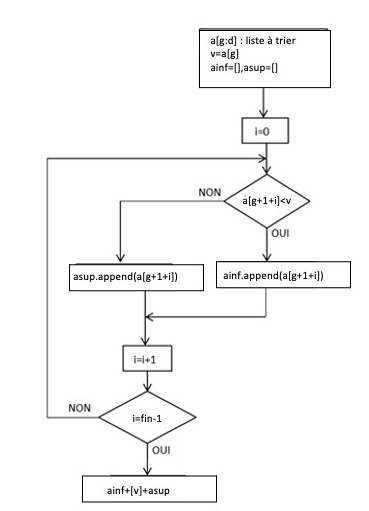
\includegraphics[width=0.9\textwidth]{algorigramme_rapide.jpg}
%\caption{Algorigramme du tri par insertion}
%\end{center}
%\end{minipage}
%\end{figure}
%
%%\begin{algorithme}[Algorithme de partitionnement pour le tri rapide]
%%
%%\begin{center}
%%		\lstinputlisting{./programmes/partition.py}
%%\end{center}
%%
%%\end{algorithme}
%
%

%La fonction tri rapide est alors implémentée de façon récursive.
%\begin{itemize}
%\item On utilise pour cela une fonction \texttt{tri\_rapide} qui prend les même arguments que la fonction \texttt{partition}.
%\item \textbf{Si} \textbf{$g\geq d-1$}, il y a au plus un élément à trier donc rien à faire (initialisation de la récursivité),
%\item \textbf{Sinon} il faut
%\begin{itemize}
%\item partitionner les élément entre \textbf{$g$} et \textbf{$d$},
%\item faire un appel récursif pour trier $a[g\cdots m[$ (partie gauche),
%\item faire un appel récursif pour trier $a[m+1\cdots d[$ (partie droite),
%\end{itemize} 
%\end{itemize} 



%Pour trier un tableau il suffit d'appeler \texttt{tri\_rapide} sur la totalité des éléments.
%

%
%%\begin{exemple2}[Algorithme complet du tri rapide avec affichage des tris successifs]
%%
%%
%%\begin{center}
%%		\lstinputlisting{./programmes/trie_rapide.py}
%%\end{center}
%%
%%\end{exemple2}
%
%
\subsubsection{Terminaison}

Prenons comme variant la longueur $n$ de la liste à trier.  Nous cherchons à trier des listes de tailles supérieure à $n$. 

Initialement, \texttt{L} est de taille \texttt{n} supérieur ou égal à 1. \texttt{n} est un entier strictement positif. 

Considérons qu'au début du ième appel de \texttt{tri\_rapide} \texttt{Li} est de taille \texttt{ni} strictement positif.

\texttt{ei} est de taille strictement inférieure à \texttt{Li} car elle ne contient que les valeurs strictement inférieures au pivot.  

\texttt{es} est de taille strictement inférieure à \texttt{Li} car elle ne contient que les valeurs supérieures ou égales au pivot, à l'exception du pivot lui-même. 

L'appel à \texttt{tri\_rapide} se fait alors sur des listes de tailles strictement inférieures à \texttt{Li}.

\texttt{n} est donc un variant de boucle et la fonction termine. 


\subsubsection{Correction}
Montrons la propriété suivante : << si \texttt{L} une liste de taille \texttt{inférieure ou égale} à $n$ alors  \texttt{tri\_rapide(L)} renvoie une liste triée >>.

\textbf{Initialisation}
La propriété de récurrence est vraie pour une liste vide et pour une liste de taille 1.

\textbf{Hérédité}
Soit une liste de taille \texttt{n+1}. Le pivot est alors \texttt{L[-1]}. \texttt{ei} et \texttt{es} ont une taille inférieure ou égale à $n$. 
D'après la proprité de récurrence, \texttt{tri\_rapide(ei)} et \texttt{tri\_rapide(es)} trient donc \texttt{ei} et \texttt{es}.

De plus, \texttt{tri\_rapide(ei) + [p] + tri\_rapide(es)} renvoie une liste triée. 

La propriété de récurrence est donc vraie pour une liste de taille \texttt{n+1}.

\subsubsection{Complexité}
\begin{prop}[Efficacité de l'algorithme]
\begin{itemize}
\item Cette méthode de tri est très efficace lorsque les données sont distinctes et non ordonnées. La complexité est alors globalement en $\mathcal{O}(n \ln(n))$. Lorsque le nombre de données devient petit (<15) lors des appels récursifs de la fonction de tri, on peut avantageusement le remplacer par un tri par insertion dont la complexité est linéaire lorsque les données sont triées ou presque. \cite{Beynet}




\item D'autre part si le tableau est déjà trié avec le code mis en place on tombe sur la complexité << dans le pire des cas >>. Une solution simple consiste à ne pas choisir systématiquement
le premier élément du segment comme pivot, mais plutôt un élément au hasard. On peut par exemple choisir la valeur de façon aléatoire. \cite{wack}
\end{itemize}

\begin{center}
\begin{tabular}{llll}
\hline
Meilleur des cas : $n \log n$ &&&  Pire des cas $n^2$  \\ 
\hline 
\end{tabular} 
\end{center}

\end{prop}


Pour un tableau de longueur $n$ :
\begin{itemize}
\item on crée une liste \texttt{ei} avec $k$ éléments et une liste \texttt{es} avec $n-k-1$ éléments (le dernier élément étant le pivot);
\item la création de chacune de ces listes fait appel à \texttt{n} comparaisons (boucles \texttt{for} qui itèrent sur chaque élément de \texttt{L});
\item on appelle alors récursivement la fonction \texttt{tri\_rapide} avec les listes de tailles précitées. 
\end{itemize} 
Le nombre de comparaisons à l'itération $n$ est donc approximativement de : 
$C(n)=2n + C(k) + C(n-k-1)$. 

Dans le pire des cas, $k=0$ (ou $k=n-1$). En conséquences,  $C(n)=2n + C(0) + C(n-1)$. Pour une liste de taille 0 ou 1, l'algorithme de tri est réalisé en un tant constant $C(0)=C(1)=1$.  

On a donc $C(n)=2n + 1 + C(n-1) \Leftrightarrow C(n)- C(n-1)=2n + 1 $. De même à l'itération $i$, on a $ C(i)- C(i-1)=2i + 1 $. 


Par sommation, on a alors :
$\sum_{i=1}^n \left(C(i)- C(i-1)\right)$
$=\sum_{i=1}^n \left(2i + 1\right) \Rightarrow C(n)-C(0) $
$= 2 \times \dfrac{1}{2} n (n+1) + n \Rightarrow C(n)=n^2 +2n -1 = \mathcal{O}(n^2)$.

%\begin{center}
%\begin{tabular}{|c|c|c|}
%\hline
%\multicolumn{3}{|c|}{\textbfComplexité}}
%\hline 
%& meilleur cas & pire cas \\ 
%\hline 
%comparaisons & $N log N$  & $N^2/2$ \\ 
%\hline 
%\end{tabular} 
%\end{center}





%%\subsection{Complexité \cite{wack}}
%%
%%
%%Pour ce calcul de complexité nous ne considérerons ici que les comparaisons. 
%%
%%La fonction partition fait toujours exactement $d-g-2$ comparaisons. Si la fonction
%%partition détermine un segment de longueur $K$ et un autre de longueur $N-1-K$, la fonction
%%$tri\_rapide$ va donc effectuer $N-1$ comparaisons par l'intermédiaire de partition,
%%puis d'autres comparaisons par l'intermédiaire des deux appels récursifs à $tri\_rapide$.
%%
%%\begin{itemize}
%%\item \textbf{Le pire des cas} correspond à $K = 0$, ce qui donne, en notant $C(N)$ la complexité du tri d'un tableau
%%de longueur $N$, l'équation de récurrence suivante:
%%
%%$$C(N) = N-1 + C(N-1)$$,
%%
%%Avec $C(1)=0$
%%
%%d'où $C(N) \sim \frac{N\times(N-1)}{2}$
%%
%%\item \textbf{Le meilleur des cas} correspond à un segment coupé en deux moitiés
%%égales, c'est-à-dire $K = N/2$. L'équation de récurrence devient : 
%%
%%$$C(N) = N-1 + 2C(N/2).$$
%%
%%
%%On peut montrer que $C(N) \sim N log N$.
%%\end{itemize} 
%%
%%
%%
%%\begin{center}
%%\begin{tabular}{|c|c|c|}
%%\hline 
%%\rule[-1ex]{0pt}{2.5ex}  & meilleur cas & pire cas \\ 
%%\hline 
%%\rule[-1ex]{0pt}{2.5ex} comparaisons & $N log N$  & $N^2/2$ \\ 
%%\hline 
%%\end{tabular} 
%%\end{center}
%%
%
%
\subsection{Tri fusion -- \textit{Merge sort}}

\subsubsection{Principe}


Cet algorithme fait aussi partie des algorithmes << diviser pour régner >>.

Le principe consiste à couper le tableau de départ en deux. On trie chacun des groupes indépendamment. Puis on fusionne les deux groupes en utilisant le fait que chacun des groupe est déjà ordonné.

Il est possible pour réaliser l'ordonnancement de chacun des groupes d'utiliser à nouveau l'algorithme de tri de façon récursive.

%
%\begin{exemple2}[Illustration sur l'exemple]
%
%
%On représente en rouge le groupe de gauche, en jaune le groupe de droite, en bleu la valeur testée du groupe de gauche et en gris la valeur testée du groupe de droite. Les valeurs en vert sont les valeurs définitivement triées.
%
%On notera que pour chaque étape, on utilise deux tableaux, le tableau de départ sur la ligne supérieure et le tableau d'arrivée sur la ligne inférieure.
%
%
%\noindent\begin{tabular}{|p{10.cm}|cccccc|}
%\hline \rowcolor{white}
%Tableau $T$ initial: On découpe en une deux moitiés (rouge et jaune). & \cellcolor{rougec}5 & \cellcolor{rougec}14 & \cellcolor{rougec}11 & \cellcolor{jaune}8 & \cellcolor{jaune}17 & \cellcolor{jaune}7 \\ 
%\hline 
%\hline \rowcolor{white}
%Chacune de ces deux listes est triée de façon indépendante (pas illustré ici) soit par un autre algorithme soit de façon récursive. & \cellcolor{rougec}5  & \cellcolor{rougec}11 &\cellcolor{rougec} 14 & \cellcolor{jaune}7 & \cellcolor{jaune}8 & \cellcolor{jaune}17  \\ 
%\hline 
%\hline 
%\rowcolor{white}
% & \cellcolor{bleuc}5  & \cellcolor{rougec}11 &\cellcolor{rougec} 14 & \cellcolor{gris25}7 & \cellcolor{jaune}8 & \cellcolor{jaune}17 \\ \cline{2-3} \rowcolor{white}
% \multirow{-2}{10.cm}{On procède alors à l'opération de fusion en comparant les premiers nombres de chaque bloc. On a besoin d'un second tableau que l'on}
%&& &  &  & &  \\
%\hline 
%\hline 
%\rowcolor{white}
%  &   & \cellcolor{rougec}11 &\cellcolor{rougec} 14 & \cellcolor{gris25}7 & \cellcolor{jaune}8 & \cellcolor{jaune}17   \\ \cline{2-3} \rowcolor{white}
% \multirow{-2}{10.cm}{remplit après les comparaisons successives des éléments des listes $L_1$ (rouge) et $L_2$ (jaune). 5<7 on le stocke de façon définitive dans $T_2$.}
%&\cellcolor{bleuc}5& &  &  & &  \\
%\hline 
%\hline 
%\rowcolor{white}
%  &   & \cellcolor{bleuc}11 &\cellcolor{rougec} 14 & \cellcolor{gris25}7 & \cellcolor{jaune}8 & \cellcolor{jaune}17   \\ \cline{2-3} \rowcolor{white}
% \multirow{-2}{10.cm}{On continue la fusion en comparant les premiers nombres restants dans chaque bloc (ici 7 et 11).}
%&\cellcolor{vertc}5& &  &  & &  \\
%\hline 
%\hline 
%\rowcolor{white}
%  &   & \cellcolor{bleuc}11 &\cellcolor{rougec} 14 &  & \cellcolor{jaune}8 & \cellcolor{jaune}17   \\ \cline{2-3} \rowcolor{white}
% \multirow{-2}{10.cm}{7<11 on le stocke dans le deuxième tableau.}
%&\cellcolor{vertc}5&\cellcolor{gris25}7 &  &  & &  \\
%\hline 
%\hline 
%\rowcolor{white}
%  &   & \cellcolor{bleuc}11 &\cellcolor{rougec} 14 &  & \cellcolor{gris25}8 & \cellcolor{jaune}17   \\ \cline{2-3} \rowcolor{white}
% \multirow{-2}{10.cm}{On continue la fusion en comparant les premiers nombres restants dans chaque bloc (8 et 11).}
%&\cellcolor{vertc}5&\cellcolor{vertc}7 &  &  & &  \\
%\hline 
%\hline 
%\rowcolor{white}
%  &   & \cellcolor{bleuc}11 &\cellcolor{rougec} 14 &  &  & \cellcolor{jaune}17   \\ \cline{2-3} \rowcolor{white}
% \multirow{-2}{10.cm}{8<11 on le stocke dans le deuxième tableau.}
%&\cellcolor{vertc}5&\cellcolor{vertc}7 &\cellcolor{gris25}8  &  & &  \\
%\hline 
%\hline 
%\rowcolor{white}
%  &   & \cellcolor{bleuc}11 &\cellcolor{rougec} 14 &  &  & \cellcolor{gris25}17   \\ \cline{2-3} \rowcolor{white}
% \multirow{-2}{10.cm}{On continu la fusion en comparant les premiers nombres restants dans chaque bloc (11 et 17).}
%&\cellcolor{vertc}5&\cellcolor{vertc}7 &\cellcolor{vertc}8  &  & &  \\
%\hline 
%\hline 
%\rowcolor{white}
%  &   &  &\cellcolor{rougec} 14 &  &  & \cellcolor{gris25}17   \\ \cline{2-3} \rowcolor{white}
% \multirow{-2}{10.cm}{11<17 on le stocke dans le deuxième tableau.}
%&\cellcolor{vertc}5&\cellcolor{vertc}7 &\cellcolor{vertc}8  &\cellcolor{bleuc}11  & &  \\
%\hline 
%\hline 
%\rowcolor{white}
%  &   &  &\cellcolor{bleuc} 14 &  &  & \cellcolor{gris25}17   \\ \cline{2-3} \rowcolor{white}
% \multirow{-2}{10.cm}{On continue la fusion en comparant les premiers nombres restants dans chaque bloc (14 et 17).}
%&\cellcolor{vertc}5&\cellcolor{vertc}7 &\cellcolor{vertc}8  & \cellcolor{vertc}11  & &  \\
%\hline 
%\hline 
%\rowcolor{white}
%  &   &  & &  &  &    \\ \cline{2-3} \rowcolor{white}
% \multirow{-2}{10.cm}{14<17 on le stocke dans le deuxième tableau et comme c'est le dernier restant on ajoute 17.}
%&\cellcolor{vertc}5&\cellcolor{vertc}7 &\cellcolor{vertc}8  &\cellcolor{rougec}11  &\cellcolor{bleuc} 14 & \cellcolor{gris25}17  \\
%\hline 
% 
%\end{tabular} 
%
%\end{exemple2}



\subsection{Implémentation}

Le tri fusion d'une liste se base sur le principe suivant : 
\begin{enumerate}
\item on sépare la liste en 2 listes de longueurs quasi-égales (à un élément près);
\item on trie ces deux listes en utilisant le tri fusion (par un appel récursif);
\item à partir de deux listes triées, on les fusionne en une seule liste en conservant l'ordre croissant.
\end{enumerate}


\begin{lstlisting}
def separe(L: list) -> tuple[list,list]:
    return L[:len(L) // 2], L[len(L) // 2:]

def fusion(L1: list, L2: list) -> list:
    """
    Fusion de deux listes triées. 
    """
    if not L1 or not L2: # si l'une des listes est vide (éventuellement les 2)
        return L1 or L2 # alors on renvoie l'autre (éventuellement vide aussi)
    else:
        a, b = L1[0], L2[0] 
        if a < b : # sinon on compare leurs premiers éléments
            return [a] + fusion(L1[1:], L2) # on place le plus petit en tête et on fusionne le reste
        else:
            return [b] + fusion(L1, L2[1:])
        
def tri_fusion(L: list) -> list:
    if len(L) < 2: # cas d'arrêt
        return L
    L1, L2 = separe(L) # sinon on sépare
    return fusion(tri_fusion(L1), tri_fusion(L2)) # et on fusionne les sous-listes triées
\end{lstlisting}
%\begin{center}
%		\lstinputlisting{./programmes/tri_fusion_recursif.py}
%\end{center}
%
%
%\begin{exemple2}[Algorithme complet du tri par fusion]
%
%
%\begin{center}
%		\lstinputlisting{./programmes/tri_fusion.py}
%\end{center}
%
%
%\end{exemple2}
%
%%
%%
%\subsection{Complexité}
%%
%%
%%%Si on note $C(N)$ (resp. $f(N)$) le nombre total de comparaisons effectuées par $tri\_fusion$
%%%(resp. fusion) pour trier un tableau de longueur $N$, on a l'équation de récurrence
%%%
%%%$$C(N) = 2C(N/2) + f(N)$$
%%%
%%%car les deux appels récursifs se font sur deux segments de même longueur $N/2$. 
%%
%%\begin{itemize}
%%\item \textbf{Dans le meilleur des cas}, la fonction fusion n'examine que les éléments de l'un des deux segments
%%car ils sont tous plus petits que ceux de l'autre segment. Dans ce cas $f(N) = N/2$ et donc
%%$C(N) \sim \frac{1}{2} N log N$. 
%%
%%\item \textbf{Dans le pire des cas}, tous les éléments sont examinés par $fusion$ et
%%donc $f(N) = N-1$, d'où $C(N) \sim N logN$.
%%\end{itemize}
%%
%%

\subsubsection{Terminaison}
\textbf{Terminaison de la fusion}
Soit la suite définie par la somme successive des longueur de \texttt{L1} et \texttt{L2}.  	 

À chaque itération on appelle \texttt{fusion} à des listes dont la taille d'une d'entre elle est diminuée de 1. La somme des longueurs est donc une suite d'entiers strictement décroissante. 

La somme des longueurs est donc un vairant de boucle et la fonction termine. 

\textbf{Terminaison du tri}

Le tri fusion termine si les listes ont 0 ou 1 éléments. 
On note $\left(u_n\right)$ la suite définie par $u_0=n$, taille de la liste à trier et $u_i$ longueur de la plus grande des listes. À chaque étape, la taille des listes est divisé par 2; donc $u_{i+1} = \left\lfloor\dfrac{u_i +1 }{2}\right\rfloor$. En conséquence, $u_{i+1}<u_i$ tant que $u_i>1$.  La fonction \texttt{tri\_fusion} termine donc. 



\subsubsection{Correction}

\subsubsection{Complexité}

\begin{prop}[Efficacité de l'algorithme]

La complexité est \textbf{$n\log(n)$} dans le meilleur des cas et dans le pire des cas.

\end{prop}

\paragraph{Complexité du tri fusion -- Petites remarques}

Quel est le coût de l'algorithme de fusion présenté précédemment ?
En Python, concaténer deux listes nécessite de copier ces deux listes dans une nouvelle liste. Cette opération est donc en $\mathcal{O}(n)$. 

Par ailleurs, la taille des listes à concaténer diminue de 1 à chaque itération. Il y aura donc $n$ appels récursifs. 

L'algorithme de fusion présenté est donc en $\mathcal{O}(n^2)$.

La séparation quant à elle est complexité $\mathcal{O}\log_2(n)$ (en effet, le nombre de fois que fois qu'on peut diviser notre liste de taille $n$ en 2 listes de taille $n//2$ est à peu près de $\log(n)$.

L'algorithme proposé est donc en $\mathcal{O}\left(n^2 \log(n)\right)$... et pas en $n\log(n)$ !

Il faudrait donc rechercher un algorithme de fusion de complexité linéaire...
\paragraph{Exemple de fusion linéaire...}
\begin{lstlisting}
def fusion(L1, L2):
    L = []
    i, j = 0, 0
    while i < len(L1) and j < len(L2):
        if L1[i] < L2[j]:
            L.append(L1[i])
            i += 1
        else:
            L.append(L2[j])
            j += 1
    L += L1[i:]
    L += L2[j:]
    return L
\end{lstlisting}


\subsection{Dans Python : sort et sorted}
Les listes Python ont une méthode native \texttt{list.sort()} qui modifie les listes elles-mêmes et renvoie \texttt{None}.
%
%	\begin{DDbox}{\linewidth}
%		\begin{verbatim}
%>>> a=[25,94,89,113,67]
%>>> a.sort()
%>>> a
%25,67,89,94,113
%		\end{verbatim}
%	\end{DDbox}
%
%
%Il y a également une fonction native \texttt{sorted()} qui construit une nouvelle liste triée depuis un itérable (liste de listes, tuple, dictionnaires).
%
%	\begin{DDbox}{\linewidth}
%		\begin{verbatim}
%>>> sorted([25,94,89,113,67])
%25,67,89,94,113
%		\end{verbatim}
%	\end{DDbox}
%
%On utilise l'indice de la "colonne" à trier en utilisant la fonction \texttt{lambda} associée à \texttt{key} :
%
%
%	\begin{DDbox}{\linewidth}
%		\begin{verbatim}
%		
%>>> etudiants=[('Julie','MPS1',15),('Elio','MPS2',14),('Jules','MPS1',17),('Adam','MPS2',16)]
%>>> sorted(etudiants, key=\textbf{lambda} etudiants : etudiants[2])
%('Elio','MPS2',14),('Julie','MPS1',15),('Adam','MPS2',16),('Jules','MPS1',17)
%>>> etudiants # etudiants est inchangé
%(Julie','MPS1',15),('Elio','MPS2',14),('Jules','MPS1',17),('Adam','MPS2',16)
%		\end{verbatim}
%	\end{DDbox}
%
%
%Sans indication particulière, le tri se fait sur la première valeur puis sur la suivante dans le cas où les premières valeurs sont identiques :
%
%	\begin{DDbox}{\linewidth}
%		\begin{verbatim}
%		>>> couple=[(3,3),(3,6),(3,1)]
%>>> sorted(couple)
%(3, 1), (3, 3), (3, 6)
%>>> le tri est dit stable
%		\end{verbatim}
%	\end{DDbox}

%\section{Tri par comptage}

\subsection{Conclusion et méthodes dans Python}


%\section{Conclusion et temps}

\begin{prop}

\textsc{Distinguer par leurs complexités deux algorithmes résolvant
un même problème :}

La première étape consiste à vérifier que les algorithmes résolvent exactement le même problème.

\begin{itemize}
\item On compare la complexité en temps dans le pire des cas (préférable a l'utilisation du module Time comme ci dessous car indépendant de la machine).
\item Il faut vérifier que le pire des cas peut arriver en situation réelle
\item Penser à comparer la complexité en espace qui peut permettre de départager des algorithmes équivalents
\end{itemize}
\end{prop}


\begin{marginfigure}
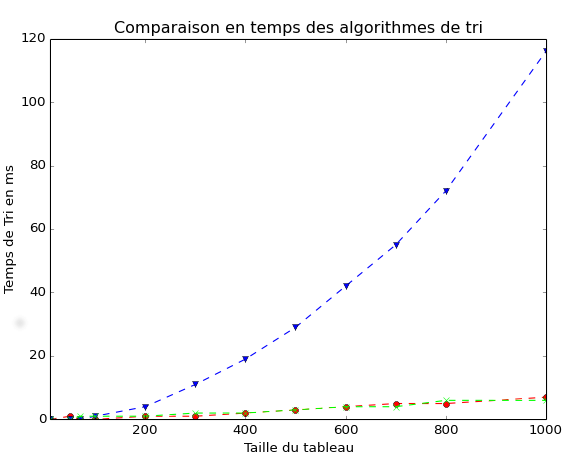
\includegraphics[width=\textwidth]{Fin.png}
\end{marginfigure}

\begin{exemple}[Illustration de la comparaison]

Pour comparer les temps globaux sur une même machine (Ici processeur	Intel Core i7-4510U Haswell (2 GHz, TDP 15W),Mémoire vive 4 Go) on génère des tableaux de dimensions différentes avec des nombres aléatoires.
On utilise le module time pour déterminer les temps. Ici c'est un temps global dépendant fortement de la machine utilisée.
On fait varier la taille du tableau et on compare les temps mis par chacun des algorithmes (en rouge tri rapide, en bleu tri insertion, en vert tri fusion). 



\end{exemple}




\begin{thebibliography}{2}

\bibitem{liesse}{Irène Charon Olivier Hudry, Algorithmes de tri, cours de Télécom ParisTech, Avril 2014.}

\bibitem{wack}{B. Wack, S. Conchon, J. Courant, M. de Falco, G. Dowek, J.-C. Filliâtre, S. Gonnord,
Informatique pour tous en classes préparatoires aux grandes écoles. Manuel
d'algorithmique et programmation structurée avec Python. Nouveaux programmes
2013. Voies MP, PC, PSI, PT, TPC et TSI, Eyrolles, 2013.}

\bibitem{Beynet}{Beynet Patrick, Cours d'informatique publié sur le site de l'UPSTI.}

\end{thebibliography}

%\section{Présentation}
%Le tri de données ou de valeurs est omniprésent en informatique. Pour cela, beaucoup d'algorithmes ont été développés afin de réaliser des tris rapidement, notamment lorsque le nombre de données est important.
%\begin{defi}\textbf{Stabilité}
%
%\end{defi}
%
%\begin{defi}\textbf{Tri en place} \\
%Un tri est effectué en place lorsque la liste à trier est modifiée jusqu'à devenir triée. Dans le cas contraire, la fonction de tri pourra renvoyer une novelle liste contenent les mêmes éléments, mais triés. 
%\end{defi}
%
%\begin{defi}\textbf{Tri comparatif} \\
%Un tri est dit comparatif lorsqu'il s'appuie uniqument sur la comparaison deux à deux des éléménts de la liste et pas sur la valeur ce ces éléments.
%\end{defi}
%
%
%\section{Tris}
%
%\begin{defi}\textbf{Tri par insertion} \\
%
%À partir d'une sous-liste triée, le tri par insertion consiste à parcourir les éléments non triés et de les insérer successivement dans la sous-liste déjà triée. 
%\end{defi}
%
%\begin{lstlisting}
%def insere(t, j):
%    k, a = j, t[j]
%    while k > 0 and a < t[k-1]:
%        t[k] = t[k-1]
%        k = k-1
%    t[k] = a
%    
%def insertionSort(t):
%    for j in range(1, len(t)):
%        insere(t, j)
%\end{lstlisting}
%
%
%\begin{defi}\textbf{Tri rapide} \\
%
%Soit une liste \texttt{L} non triée. Soit \texttt{p} un terme appelé pivot. Le tri rapide consiste à répartir les éléments strictement inférieur au pivot avant ce dernier et les termes plus grand après le pivot (segemntation). Le pivot est à ce stade trié correctement par rapport aux autres valeurs de la liste. Ce principe est alors appliqué récursivement aux deus-sous listes  séparées par le pivot.
%
%\end{defi}
%
%
%\begin{lstlisting}
%def segmente(t, i, j):
%    p = t[j-1] # On prend comme pivot le dernier élément de la sous liste. 
%    a = i
%    for b in range(i, j-1):
%        if t[b] < p:
%            t[a], t[b] = t[b], t[a]
%            a += 1
%    t[a], t[j-1] = t[j-1], t[a] # On positionne le pivot "à sa place".
%    return a # On retourne l'index du pivot. Le tableau a été modifié en place. 
%\end{lstlisting}
%
%\begin{lstlisting}
%def quickSort(t, i, j):
%    if i + 1 < j:
%        a = segmente(t, i, j)
%        quickSort(t, i, a)
%        quickSort(t, a + 1, j)
%\end{lstlisting}
%
%\begin{lstlisting}
%# Instruction pour trier une liste
%quickSort(t, 0, len(t))
%\end{lstlisting}
%\begin{defi}\textbf{Tri fusion} \\
%Il s'agit d'un tri s'appuyant sur la stratégie divisér pour régner. 
%
%L'algorithme est le suivant : 
%\begin{itemize}
%\item on divise la liste en deux listes de tailles quasi-identiques;
%\item on trie récursivement ces deux listes;
%\item on fusionne les deux listes triées.
%\end{itemize}
%\end{defi}
%
%\begin{lstlisting}
%def placer(L :list, p :int, x) :
%    """Place un élément x à sa place dans une liste L triée à partir de l'indice p
%    Entrée :
%        L : une liste, p : un entier, x : un élément
%    Sorties :
%        La liste est modifiée mais n'est pas renvoyée. k la valeur de l'indice de la liste où l'élément a été placé"""
%    k = p
%    while ( k < len(L) and x > L[k]) :
%        k = k+1
%    L.insert(k, x)
%    return k
%    
%def fusion(a:list, b:list) :
%    """Fusionne les deux listes
%    Entrée : deux listes a et b triées.
%    Sortie : La liste b modifiée"""
%    p = 0
%    for x in a :
%        p = placer(b, p, x)+1
%    return b
%
%def tri_fusion(t : list) :
%    """Trie la liste t
%    Entrée : une liste.
%    Sortie : la liste est modifiée."""
%    if len(t) < 2 :
%        return (t)
%    else :
%        m = len(t) // 2
%        return (fusion (tri_fusion(t[:m]) , tri_fusion(t[m:]) ))
%\end{lstlisting}
%
%\begin{proposition}\textbf{Complexité des algorithmes}
%On note $T(n)$ le nombre de comaraisons nécessaire pour trier une liste de longueur $n$. 
%On montre que dans le pire des cas, les complexités sont les suivantes :
%\begin{itemize}
%\item tri par insertion : $T_{\text{Max}}(n)=\mathcal{O}\left(n^2\right)$;
%\item tru rapide : $T_{\text{Max}}(n)=\mathcal{O}\left(n^2\right)$;
%\item tru partition-fusion : $T_{\text{Max}}(n)=\mathcal{O}\left(n\log n\right)$.
%\end{itemize}
%
%
%
%\end{proposition}
%
%
%
%
%\section{Acticité préparatoire}
%\textbf{Pour réaliser l'activité associée à ce cours, suivre le lien suivant : }
%\begin{itemize} 
%\item Sujet : \url{https://bit.ly/3iAc5do}
%\item Corrige : \url{https://bit.ly/3eFuHrt}
%\end{itemize}
%
%\section{QCM}
%\begin{multicols}{2}
%\question{On dispose d'une liste de triplets: t = [(1,12,250),(1,12,251), (2,12,250),(2,13,250),(2,11,250),(2,12,249)].
%On trie cette liste par ordre croissant des valeurs du second élément des triplets. En cas d'égalité, on trie par ordre croissant du troisième champ. Si les champs 2 et 3 sont égaux, on trie par ordre croissant du premier champ.
%Après ce tri, quel est le contenu de la liste ?}
%\begin{enumerate}
%\item \texttt{[(1,12,249),(1,12,250),(1,12,251),(2,11,250),(2,12,250),(2,13,250)]}.
%\item \texttt{[(2,11,250),(1,12,249),(1,12,250),(2,12,250),(1,12,251),(2,13,250)]}.%+
%\item \texttt{[(2,11,250),(1,12,249),(1,12,250),(1,12,251),(2,12,250),(2,13,250)]}.
%\item \texttt{[(1,12,249),(2,11,250),(1,12,250),(2,12,250),(2,13,250),(1,12,251)]}.
%\end{enumerate}
%
%\question{Quelle valeur retourne la fonction \texttt{mystere} suivante ?}
%\begin{lstlisting}
%def mystere(liste):
%     valeur_de_retour = True
%     indice = 0
%     while indice < len(liste) - 1 :
%          if liste[indice] > liste[indice + 1]:
%               valeur_de_retour = False
%          indice = indice + 1
%     return valeur_de_retour
%\end{lstlisting}
%\begin{enumerate}
%\item Une valeur booléenne indiquant si la liste liste passée en paramètre est triée. %+
%\item La valeur du plus grand élément de la liste passée en paramètre.
%\item La valeur du plus petit élément de la liste passée en paramètre.
%\item Une valeur booléenne indiquant si la liste passée en paramètre contient plusieurs fois le même élément.
%\end{enumerate}
%
%\question{Combien d'échanges effectue la fonction Python suivante pour trier un tableau de 10 éléments au pire des cas ?}
%\begin{lstlisting}
%def tri(tab) :
%     for i in range (1, len(tab)) :
%          for j in range (len(tab) - i) :
%               if tab[j] > tab[j+1] :
%                    tab[j], tab[j+1] = tab[j+1], tab[j]
%\end{lstlisting}
%\begin{enumerate}
%\item 45. %+
%\item 100.
%\item 10.
%\item 55.
%\end{enumerate}
%
%\question{Que vaut l'expression \texttt{f([7, 3, 1, 8, 19, 9, 3, 5], 0)} ?}
%\begin{lstlisting}
%def f(t,i) :
%     im = i
%     m = t[i]
%     for k in range(i+1, len(t)) :
%          if t[k] < m :
%               im, m = k, t[k]
%     return im
%\end{lstlisting}
%\begin{enumerate}
%\item 1.
%\item 2. %+
%\item 3.
%\item 4.
%\end{enumerate}
%
%\question{Laquelle de ces listes de chaînes de caractères est triée en ordre croissant ?}
%\begin{lstlisting}
%\end{lstlisting}
%\begin{enumerate}
%\item \texttt{['Chat' , 'Cheval' , 'Chien' , 'Cochon']}. %+
%\item \texttt{['Cochon' , 'Chat' , 'Cheval' , 'Chien']}.
%\item \texttt{['Cheval' , 'Chien‘ , 'Chat' , 'Cochon']}.
%\item \texttt{['Chat' , 'Cochon' , 'Cheval' , 'Chien']}.
%\end{enumerate}
%
%\question{Laquelle de ces listes de chaînes de caractères est triée en ordre croissant ?}
%\begin{lstlisting}
%\end{lstlisting}
%\begin{enumerate}
%\item \texttt{['12','142','21','8']}. %+
%\item \texttt{['8','12','142','21']}.
%\item \texttt{['8','12','21','142']}.
%\item \texttt{['12','21','8','142']}.
%\end{enumerate}
%
%\question{Quelle est la valeur de la variable \texttt{table} après exécution du programme Python suivant ?}
%\begin{lstlisting}
%table = [12, 43, 6, 22, 37]
%for i in range(len(table) - 1):
%    if table [i] > table [i+1] :
%        table [i] ,table [i+1] = table [i+1] ,table [i]
%\end{lstlisting}
%\begin{enumerate}
%\item \texttt{[12, 6, 22, 37, 43]}.%+
%\item \texttt{[6, 12, 22, 37, 43]}.
%\item \texttt{[43, 12, 22, 37, 6]}.
%\item \texttt{[43, 37, 22, 12, 6]}.
%\end{enumerate}
%
%\question{Un algorithme cherche la valeur maximale d'une liste non triée de taille $n$. Combien de temps mettra cet algorithme sur une liste de taille $2n$ ?}
%
%\begin{enumerate}
%\item Le même temps que sur la liste de taille n si le maximum est dans la première moitié de la liste.
%\item On a ajouté $n$ valeurs, l'algorithme mettra donc n fois plus de temps que sur la liste de taille $n$.
%\item Le temps sera simplement doublé par rapport au temps mis sur la liste de taille $n$.%+
%\item On ne peut pas savoir, tout dépend de l'endroit où est le maximum.
%\end{enumerate}
%
%\question{Quel est le coût en temps dans le pire des cas du tri par insertion ?}
%
%\begin{enumerate}
%\item $\mathcal{O}(n)$.
%\item $\mathcal{O}\left(n^2\right)$.%+
%\item $\mathcal{O}\left(2^n\right)$.
%\item $\mathcal{O}\left(\log n\right)$.
%\end{enumerate}
%
%\end{multicols}
%
%%\question{On souhaite écrire une fonction \texttt{tri\_selection(t)}, qui trie le tableau \texttt{t} dans l'ordre croissant : parmi les 4 programmes suivants, lequel est correct ?}
%%\begin{lstlisting}
%%def tri_selection(t) :
%%     for i in range (len(t)-1) :
%%          min = i		
%%          for j in range(i+1,len(t)):
%%               if t[j] < t[min]:
%%                    min = j
%%          tmp = t[i]
%%          t[i] = t[min]
%%          t[min] = tmp
%%def tri_selection(t) :
%%     for i in range (len(t)-1) :
%%          min = i		
%%          for j in range(i+1,len(t)-1):
%%               if t[j] < t[min]:
%%                    min = j
%%          tmp = t[i]
%%          t[i] = t[min]
%%          t[min] = tmp
%%def tri_selection(t) :
%%     for i in range (len(t)-1) :
%%          min = i		
%%          for j in range(i+1,len(t)):
%%               if t[j] < min:
%%                    min = j
%%          tmp = t[i]
%%          t[i] = t[min]
%%          t[min] = tmp
%%def tri_selection(t) :
%%     for i in range (len(t)-1) :
%%          min = i		
%%          for j in range(i+1,len(t)):
%%               if t[j] < t[min]:
%%                    min = j
%%          tmp = t[i]
%%          t[min] = t[i]
%%          t[i] = tmp
%%\end{lstlisting}
%%\begin{enumerate}
%%\item Fonction 1. %+
%%\item Fonction 2.
%%\item Fonction 3.
%%\item Fonction 4.
%%\end{enumerate}
%%
%%\question{De quel type de tri s'agit-il ?}
%%\begin{lstlisting}
%%def tri(lst):
%%    for i in range(1,len(lst)):
%%        valeur = lst[i]
%%        j = i
%%        while j>0 and lst[j-1]>valeur:
%%            lst[j]=lst[j-1]
%%            j = j-1
%%        lst[j]=valeur
%%\end{lstlisting}
%%\begin{enumerate}
%%\item Tri par insertion. %+
%%\item Tri fusion.
%%\item Tri par sélection.
%%\item Tri à bulles.
%%\end{enumerate}
%%
%%\question{De quel type de tri s'agit-il ?}
%%\begin{lstlisting}
%%def tri(lst):
%%    nb = len(lst)
%%    for i in range(0,nb):    
%%        ind_plus_petit = i
%%        for j in range(i+1,nb) :
%%            if lst[j] < lst[ind_plus_petit] :
%%                ind_plus_petit = j
%%        if ind_plus_petit is not i :
%%            temp = lst[i]
%%            lst[i] = lst[ind_plus_petit]
%%            lst[ind_plus_petit] = temp
%%\end{lstlisting}
%%\begin{enumerate}
%%\item Tri par insertion. 
%%\item Tri fusion.
%%\item Tri par sélection. %+
%%\item Tri à bulles.
%%\end{enumerate}
%%
%%\question{Un algorithme est en complexité quadratique. Codé en python, son exécution pour des données de taille 100 prend 12 millisecondes. Si l'on fournit des données de taille 200 au programme, on peut s'attendre à un temps d'exécution d'environ :}
%%\begin{lstlisting}
%%\end{lstlisting}
%%\begin{enumerate}
%%\item 48 millisecondes. %+
%%\item 24 millisecondes.
%%\item 12 millisecondes.
%%\item 96 millisecondes.
%%\end{enumerate}
%%
%%\question{À quel type tri correspond l'invariant de boucle ci-dessous :}
%%\begin{itemize}
%%\item tous les éléments d'indices 0 à $i-1$ sont déjà triés,
%%\item tous les éléments d'indices $i$ à $n$ sont de valeurs supérieures à ceux de la partie triée.
%%\end{itemize}
%%\begin{enumerate}
%%\item Tri par insertion. 
%%\item Tri fusion.
%%\item Tri par sélection. %+
%%\item Tri à bulles.
%%\end{enumerate}
%%
%%\question{Quel est l'invariant de boucle qui correspond précisément à cet algorithme ?}
%%
%%On considère un algorithme de tri par sélection, dans lequel la fonction \texttt{echanger(tab[i], tab[j])}
%%effectue l'échange des ième et jième valeurs du tableau \texttt{tab}.
%%\begin{lstlisting}
%%nom: tri_sélection
%%
%%paramètre: tab, tableau de n entiers, n>=2
%%
%%Traitement:
%%pour i allant de 1 à n-1:
%%    pour j allant de i+1 à n:
%%        si tab[j] < tab[i]:
%%            echanger(tab[i], tab[j])
%%renvoyer tab
%%\end{lstlisting}
%%\begin{enumerate}
%%\item Tous les éléments d'indice supérieur ou égal à i sont triés par ordre croissante.
%%\item Tous les éléments d'indice compris entre 0 et i sont triés et les éléments d'indice supérieurs ou égal à i leurs sont tous supérieurs.
%%\item Tous les éléments d'indice supérieur ou égal à i sont non triés.
%%\item Tous les éléments d'indice compris entre 0 et i sont triés, on ne peut rien dire sur les éléments d'indice supérieur ou égal à i.
%%\end{enumerate}
%%
%%\question{Quel est le type de tri qui correspond à cet algorithme ?}
%%\begin{lstlisting}
%%nom: tri_mystere
%%
%%paramètre: tab, tableau de n entiers, non trié, non vide
%%
%%Traitement:
%%pour i allant de 1 à n-1:
%%    pour j allant de i+1 à n:
%%        si tab[j] < tab[i]:
%%            echanger(tab[i], tab[j])
%%renvoyer tab
%%\end{lstlisting}
%%\begin{enumerate}
%%\item Tri par insertion. 
%%\item Tri fusion.
%%\item Tri par sélection. %+
%%\item Tri rapide.
%%\end{enumerate}
%%
%%\question{Quel est l'invariant de boucle qui correspond précisément à cet algorithme ?}
%%\begin{lstlisting}
%%nom: tri_insertion
%%
%%paramètre: tab, tableau de n entiers, n >= 2
%%
%%Traitement:
%%pour i allant de 2 à n:
%%    j = i
%%    tant que j > 1  et tab[j-1] > tab[j]:
%%        echanger(tab[j-1], tab[j])
%%        j = j-1
%%renvoyer tab
%%\end{lstlisting}
%%\begin{enumerate}
%%\item Tous les éléments d'indice compris entre 0 et i sont triés et les éléments d'indice supérieurs ou égal à i leurs sont tous supérieurs.
%%\item Tous les éléments d'indice supérieur ou égal à i sont triés par ordre croissant.
%%\item Tous les éléments d'indice compris entre 0 et i sont triés, on ne peut rien dire sur les éléments d'indice supérieur ou égal à i. %+
%%\item Tous les éléments d'indice supérieur ou égal à i sont non triés par ordre croissants.
%%\end{enumerate}
%%
%%\question{Parmi les propositions suivantes, quelle est celle qui ne correspond pas à une méthode de tri ?}
%%\begin{lstlisting}
%%\end{lstlisting}
%%\begin{enumerate}
%%\item Par sélection.
%%\item Par insertion.
%%\item Par rotation. %+
%%\item Par fusion.
%%\end{enumerate}
